\chapter{Implementation}
\label{chap:implementation}

\section{Chosen Software Architecture}
In the given setting, the most accessible frontend is commonly a JavaScript web application.

To still make the classification run as quickly and efficiently as possible, a C++ binary runs
in the backend providing an HTTP API to the frontend application.
In order to allow for more flexibility of the HTTP server, the initial approach was to
pipe requests through a dedicated web application framework with database access
that would allow, for instance, user management next to the basic classification.
However, the resulting communication and computation overhead, even when running with very
efficient protocols such as ZeroMQ, was too high.

Extending the accessibility argument to reproducibility, Docker is a very solid choice \parencite{using-docker-in-science}.
To run the attached demo project, simply execute
\begin{minted}{bash}
  docker-compose build
  docker-compose up
\end{minted}
in the 'code' folder and point your browser to \url{https://locahost}.

\section{The MNIST dataset}
The MNIST dataset \parencite{mnist-original} contains X train and Y test images with corresponding labels.
In order to stick to the traditional feedforward technique with data represented
in vector format, therefore it is common to reshape data from $(28, 28)$ images (represented as grayscale values in a matrix)
into a $784$ element vector.

\section{Matrix-Vector Multiplication}
The dot product that is required as part of the neural network evaluation process
needs to be implemented on SEAL ciphertexts as well.

There are multiple methods to achieve a syntactically correct dot product (matrix-vector multiplication)
as described by \textcite{2018-gazelle} for square matrices.

\begin{enumerate}
  \item Naive
  \item Diagonal
  \item Hybrid
\end{enumerate}

\begin{figure}
  \centering
  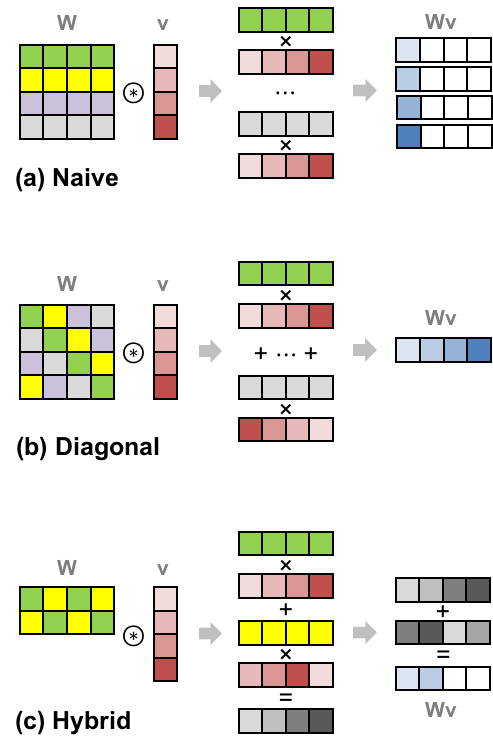
\includegraphics[width=0.4\linewidth]{figures/matrix-vector-multiplication-techniques.png}
  \caption[Image source: \cite{2018-gazelle}]{Different techniques to compute a dot product between a matrix and a vector,
    each having their up- and downsides.}
\end{figure}

\subsection{Adapting to non-square matrices}
The weight matrices in the given classification setting
are by no means square, on the contrary their output dimension tends
to be much lower than the input dimension as the goal is to reduce it from
$28^2 = 784$ to $10$ overall.

However, that also means one cannot directly apply the diagonal method
as described in the proceedings above.
This 'flaw' can be mitigated by a simple zero-padding approach
in order to make the matrix square, filling in zeros until
the lower dimension reaches the higher one.
